%!TEX program = xelatex
\documentclass[10pt,mathserif]{beamer}%,aspectratio=169 %画面比例16:9%
\usepackage{ctex}
\usepackage{xeCJK}
\usepackage{listings}
\usepackage{makecell}
\usepackage{setspace}
\usepackage{array}
\usepackage{booktabs} %调整表格线与上下内容的间隔
\usepackage{subcaption}
\usepackage[linesnumbered,slide,algoruled]{algorithm2e}
\usepackage{indentfirst}
\usepackage{multirow}
\usepackage{ulem}



\usetheme[
	sidebar, % 会在每页左侧加上导航栏,参考 The AAU Sidebar Beamer Theme 设置
	xdblue, % 不选会默认西电红色调,选上会将主题设置为西电蓝色调
	% english % 选上,会将图表等标题还原回英文标题
 ]{XDUstyle}


\title{无人机智能避障与导航}
\institute[北京航空航天大学\\计算机学院]{北京航空航天大学计算机学院23级硕士研究
生} % 中括号部分为导航栏底所用尽可能精简
\author{黄栋篪}
\date{\today}% 时间可自行设置


\setlength{\footnotesep}{0pt}
\setbeamerfont{footnote mark}{size=\tiny}
\setbeamerfont{footnote text}{size=\tiny}
\setbeamertemplate{footnote}{%
  {\setlength{\hsize}{330pt}%
   \usebeamercolor[fg]{footnote mark}%
   \usebeamerfont*{footnote mark}%
   \hspace*{1.5em}%
   \@thefnmark.~%
   \usebeamercolor[fg]{footnote text}%
   \usebeamerfont*{footnote text}%
   \insertfootnotetext\par}}
\setbeamertemplate{bibliography entry article}{}
\setbeamertemplate{bibliography entry title}{}
\setbeamertemplate{bibliography entry location}{}
\setbeamertemplate{bibliography entry note}{}
\setbeamertemplate{navigation symbols}{}
\def\beamer@newblock{%
  \usebeamercolor[fg]{bibliography entry author}%
  \usebeamerfont{bibliography entry author}%
  \usebeamertemplate{bibliography entry author}%
  \def\newblock{%
    \usebeamercolor[fg]{bibliography entry title}%
    \usebeamerfont{bibliography entry title}%
    \usebeamertemplate{bibliography entry title}%
    \def\newblock{%
      \usebeamercolor[fg]{bibliography entry location}%
      \usebeamerfont{bibliography entry location}%
      \usebeamertemplate{bibliography entry location}%
      \def\newblock{%
        \usebeamercolor[fg]{bibliography entry note}%
        \usebeamerfont{bibliography entry note}%
        \usebeamertemplate{bibliography entry note}}}}}
\makeatother
	
\begin{document}

{\xdbg \frame[plain,noframenumbering]{\titlepage}}%首页标题页

\section{overview}

\begin{frame}[fragile]
	\frametitle{overview}
	% \setlength{\parindent}{2em}
	\begin{spacing}{1.5}
		SafeDreamer Project主要分为两个部分:
		\begin{itemize}
			\item RL算法. SafeDreamer 结合了世界模型、拉格朗日约束和PPO算法的
			一种基于安全强化学习的智能导航算法
		\end{itemize}
		\begin{itemize}
			\item Safety-Gymnasium. Safety-Gymnasium是一个基于MuJoCo引擎的仿真验证环境,
			主要面向SafeRL算法的智能体仿真验证,它支持单、多智能体;基于OpenGL库,支持丰富的视觉输入;
			高度可定制化;支持多种智能体和任务;并且集成一个SafeRL算法库。
		\end{itemize}
	\end{spacing}
\end{frame}

\section{RL算法}
\begin{frame}[fragile]
	\frametitle{SafeDreamer Algorithm}
	% \setlength{\parindent}{2em}
	\begin{spacing}{1.5}
		SafeDreamer是World Model, Lagrangian SafeRL methods和CCEM三种方法的结合,最终取得了良好的效果。
		\begin{itemize}
			\item World Model.World Model 是一种用来记忆和建模环境的神经网络模块,
			在SafeDreamer中使用DreamerV3来作为World Model,其神经网络结构为RSSM.
		\end{itemize}
		\begin{itemize}
			\item Lagrangian SafeRL methods.Lagrangian SafeRL methods 是一种通过拉格朗日方法来求解强
			化学习中有约束优化问题的一种方法。在SafeDreamer中使用Lag-aug和PID-Lag来提高模型性能。
		\end{itemize}
		\begin{itemize}
			\item CCEM.约束交叉熵方法(CCEM),:在每次迭代中,首先从策略分布中取样,选择一组精英样本策略,
			并使用它们来更新策略分布。精英样本:我们使用约束值对样本策略进行排序,然后选择约束性能最好的策略。
		\end{itemize}
	\end{spacing}
\end{frame}

\subsection{Preliminaries}

\begin{frame}[fragile]
	\frametitle{World Model}
	\begin{spacing}{1.5}
		综合考虑各个仿真工具的优劣, 最终决定使用ns-3.
		\begin{itemize}
			\item 从工具的性质来说, QualNet以及Opnet均为
				\textcolor{red}{商业软件}, 并不能免费获取;而ns-3是
				\textcolor{blue}{开源软件}, 在Windows、MacOS、Linux上均
				可以免费获取和使用,便于开发.
			\item 从工具的维护情况来说, ns-3由一个活跃的社区维护, 最新版本
				ns-3.39于\textcolor{blue}{2023年7月}发布; 而Opnet在被收购前的最
				新免费版本为14.5,该版本于2012年发布, 距今已有\textcolor{red}{十
				余年}.
		\end{itemize}
	\end{spacing}
\end{frame}

\subsection{ns-3的仿真能力}

\begin{frame}[fragile]
	\frametitle{仿真工具选择}
	\begin{spacing}{1.5}
		就仿真能力而言, ns-3的优势功能如下:
		\begin{itemize}
			\item ns-3提供了一个灵活的仿真框架, 可以轻松地创建和定制各种网络拓扑
				和协议. ns-3可以对物理层、链路层、网络层等各个OSI层次进行修改和
				定制.
				\begin{itemize}
					\item 在物理层, ns-3提供了多种模型和技术, 如无线信道模型、传
						输介质模型等, 可以模拟不同类型的物理介质和信道特性.
					\item 在链路层, ns-3支持多种链路层协议和技术, 如以太网、
						Wi-Fi、LTE等. 用户可以使用现有的链路层协议模型, 也可以根
						据需要自定义新的链路层协议.
					\item 在网络层方面, ns-3支持多种网络层协议, 如IPv4、IPv6、路
						由协议(如OSPF、BGP等). 
				\end{itemize}
		\end{itemize}
	\end{spacing}
\end{frame}

\begin{frame}[fragile]
	\frametitle{仿真工具选择}
	\begin{spacing}{1.5}
		\begin{itemize}
			\item ns-3提供了丰富的可视化和分析工具, 可以帮助用户可视化仿真结果并
				进行详细的性能分析. 这些工具可以帮助用户理解网络行为、优化协议和
				算法, 并进行实验评估. 
				\begin{figure}[htb]
					\centering
					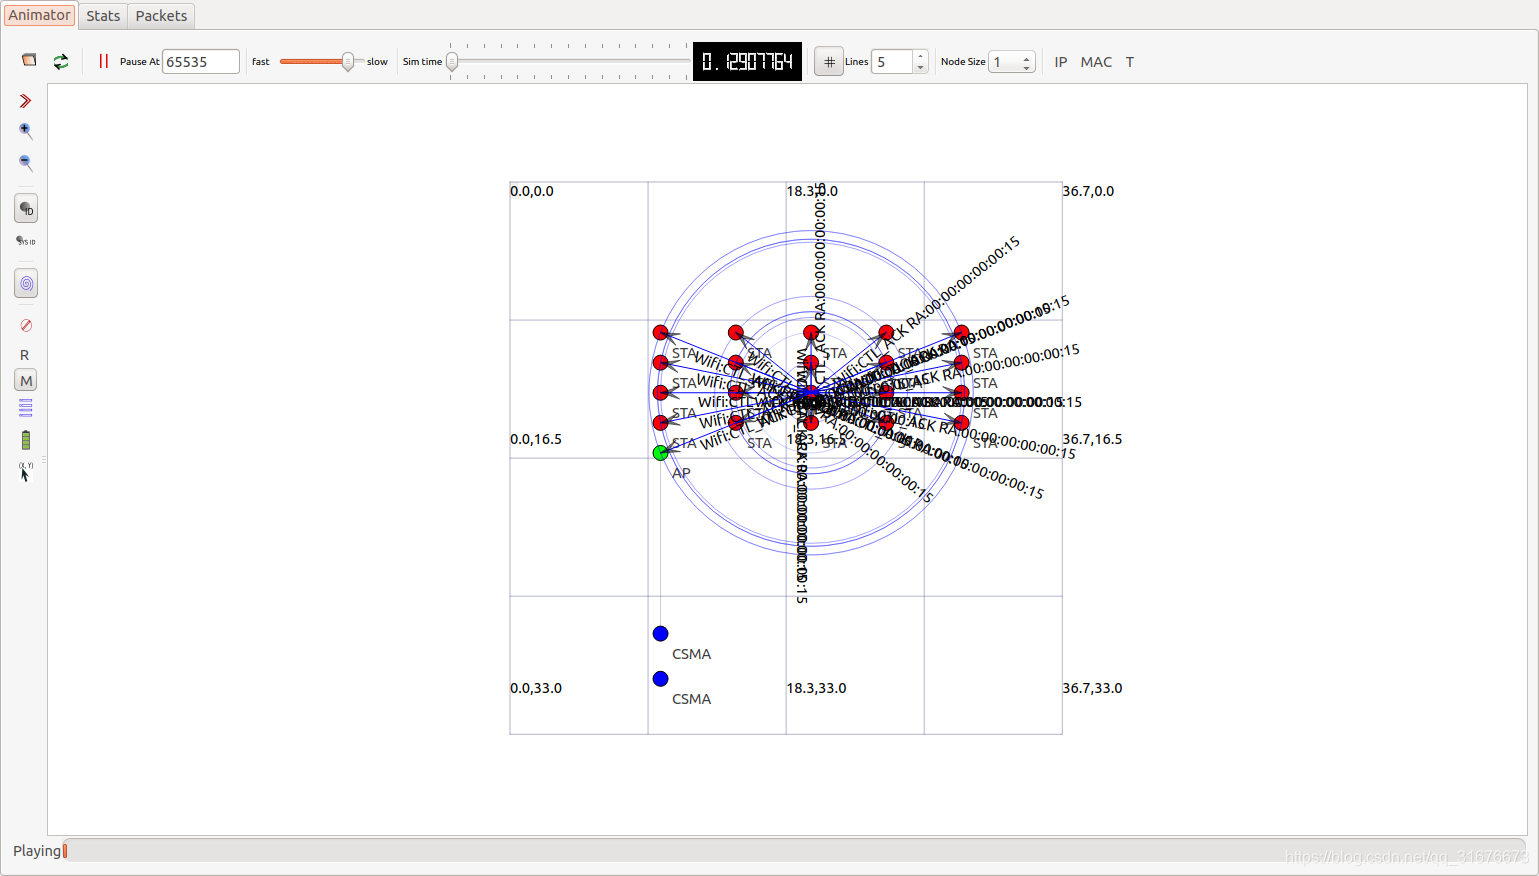
\includegraphics[width=0.9\linewidth]{./images/net.png}
					\caption{可视化工具NetAnim示意图}
					\label{Fig:net}
				\end{figure}
		\end{itemize}
	\end{spacing}
\end{frame}

\begin{frame}[fragile]
	\frametitle{仿真工具选择}
	\setlength{\parindent}{2em}
	\begin{spacing}{1.5}
		\begin{itemize}
			\item 社区支持和文档丰富: ns-3拥有一个活跃的社区, 提供了广泛的文档、
				教程和示例, 以帮助用户入门和解决问题.
				\begin{figure}[htb]
					\centering
					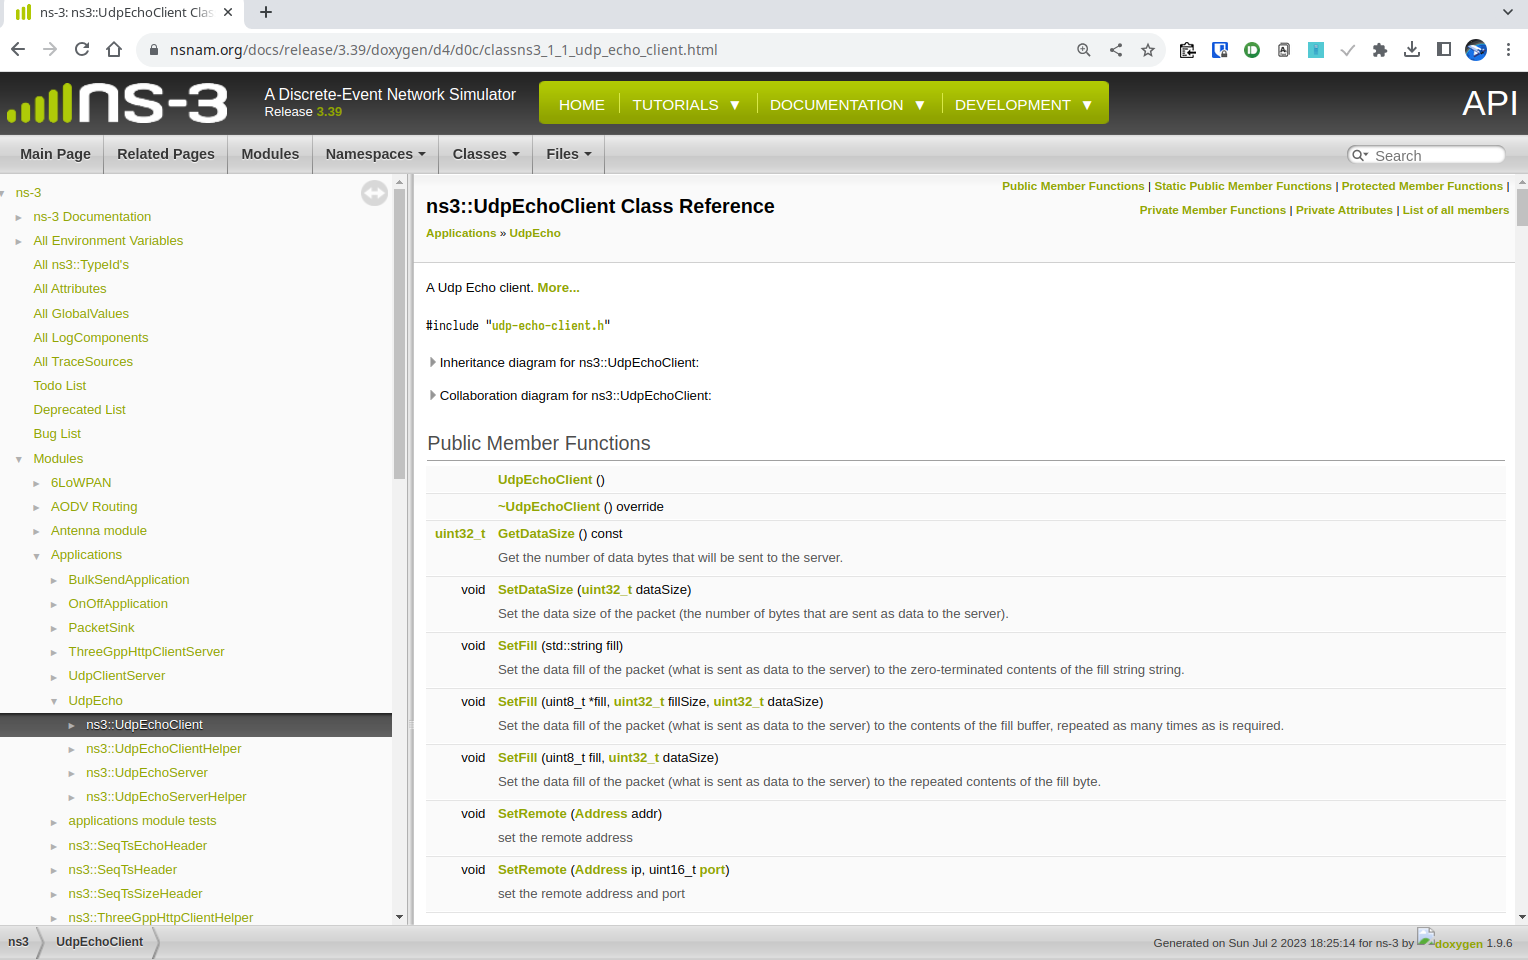
\includegraphics[width=1\linewidth]{./images/pic.png}
					\caption{ns-3详尽的API文档}
					\label{Fig:pic}
				\end{figure}
		\end{itemize}
	\end{spacing}
\end{frame}

\subsection{仿真面临的困难}
\begin{frame}[fragile]
	\frametitle{仿真工具选择}
	\setlength{\parindent}{2em}
	\begin{spacing}{1.5}
		不过基于ns-3做仿真研究也有一些不足的地方: 在中文互联网上(知网等), 绝大部
		分的数据链仿真都是使用Opnet开展的, 一小部分是使用QualNet仿真的, 只有极小
		一部分是使用ns-3做的仿真, 这极大程度上增加了仿真研究的难度.

		另一个严重的问题是, \textbf{几乎所有}有关数据链仿真的文章均未完整公开所有的代码细
		节, 只是把整个功能模块当作一个黑盒笼统地介绍给读者, 读者完全无法深入了解
		编码细节, 更无法对其仿真结果做复现; 在Github等开源平台上也完全无法找到前
		人做过的仿真工作代码.
	\end{spacing}
\end{frame}


\section{仿真内容确定}

\begin{frame}[fragile]
	\frametitle{仿真内容确定}
	\setlength{\parindent}{2em}
	\begin{spacing}{1.5}
		有关仿真内容的确定考虑以一篇国防科大的博士论文
		\cite{zhanshushujulianzuwang}为主线, 在此之上核查一下美军对数据链的官
		方标准, 并尝试对其进行仿真实现.
	\end{spacing}
\end{frame}


\subsection{战术数据链仿真平台框架}

\begin{frame}[fragile]
	\frametitle{战术数据链仿真平台框架}
	\setlength{\parindent}{2em}
	\begin{spacing}{1.5}
		\begin{figure}[htb]
			\centering
			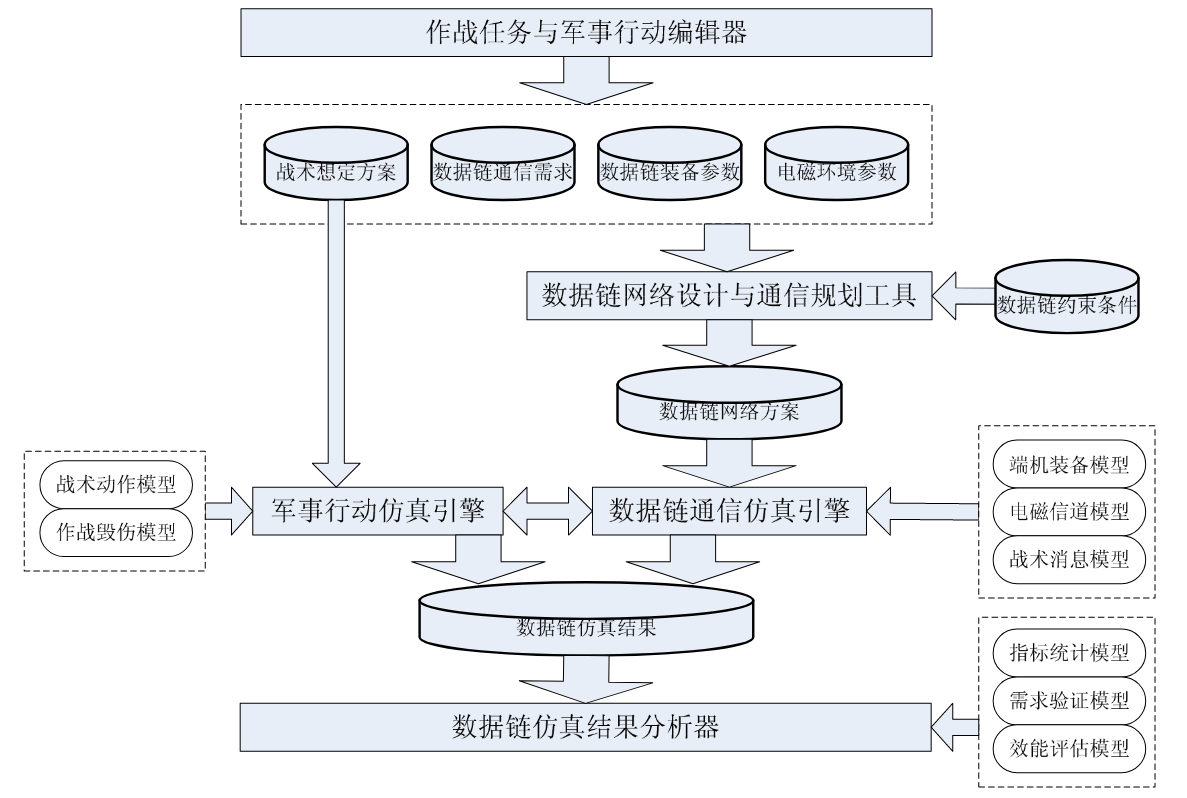
\includegraphics[width=1\linewidth]{./images/arch.png}
			\caption{战术数据链仿真平台框架结构图}
			\label{Fig:arch}
		\end{figure}
	\end{spacing}
\end{frame}

\begin{frame}[fragile]
	\frametitle{战术数据链仿真平台框架}
	% \setlength{\parindent}{2em}
	该框架主要由5个部分构成:
	\begin{spacing}{1.5}
		\begin{itemize}
			\item 作战任务与军事行动编辑器: 作战任务与军事行动是整个仿真实验的
				``剧本''. 包括初始状态, 仿真过程 中即将发生的时间及其交互等. 作
				战任务与军事行动编辑器的功能就是根据给定 的战术任务, 通过各种条
				令条例和战法战例等生成整个仿真实验所需要的规范化 的剧情. 其中主
				要包括战术想定方案的编辑、信息交换需求的确认与分析、战术 数据链
				装备平台的选择以及战场环境的生成. 
		\end{itemize}
	\end{spacing}
\end{frame}

\begin{frame}[fragile]
	\frametitle{战术数据链仿真平台框架}
	\setlength{\parindent}{2em}
	\begin{spacing}{1.5}
		\begin{figure}[htb]
			\centering
			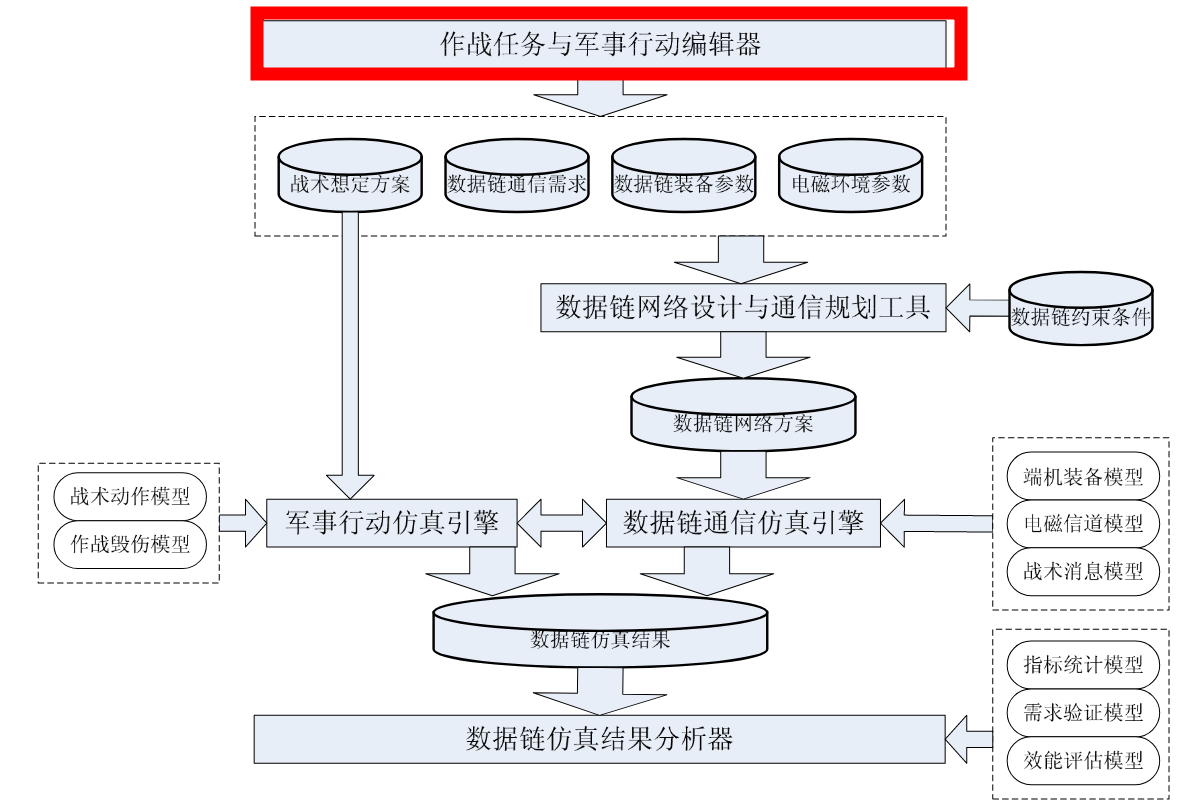
\includegraphics[width=1\linewidth]{./images/arch1.png}
		\end{figure}
	\end{spacing}
\end{frame}

\begin{frame}[fragile]
	\frametitle{战术数据链仿真平台框架}
	% \setlength{\parindent}{2em}
	\begin{spacing}{1.5}
		\begin{itemize}
			\item 战术数据链网络设计与通信规划工具: 根据若干网络资源分配规则与战
				术数据链网络角色选择方案,  保证各项信息交换需求能够得到满足, 这
				其中就包括指定并配置相 应的网络功能实现信息交换、指派合适的网络
				角色履行其网络职责以及对有限的 战术数据链网络资源进行合理分配.
				战术数据链组网设计规划工具最终生成组网 方案, 作为战术数据链通信
				仿真引擎的输入, 驱动仿真引擎的模拟仿真. 
		\end{itemize}
	\end{spacing}
\end{frame}

\begin{frame}[fragile]
	\frametitle{战术数据链仿真平台框架}
	\setlength{\parindent}{2em}
	\begin{spacing}{1.5}
		\begin{figure}[htb]
			\centering
			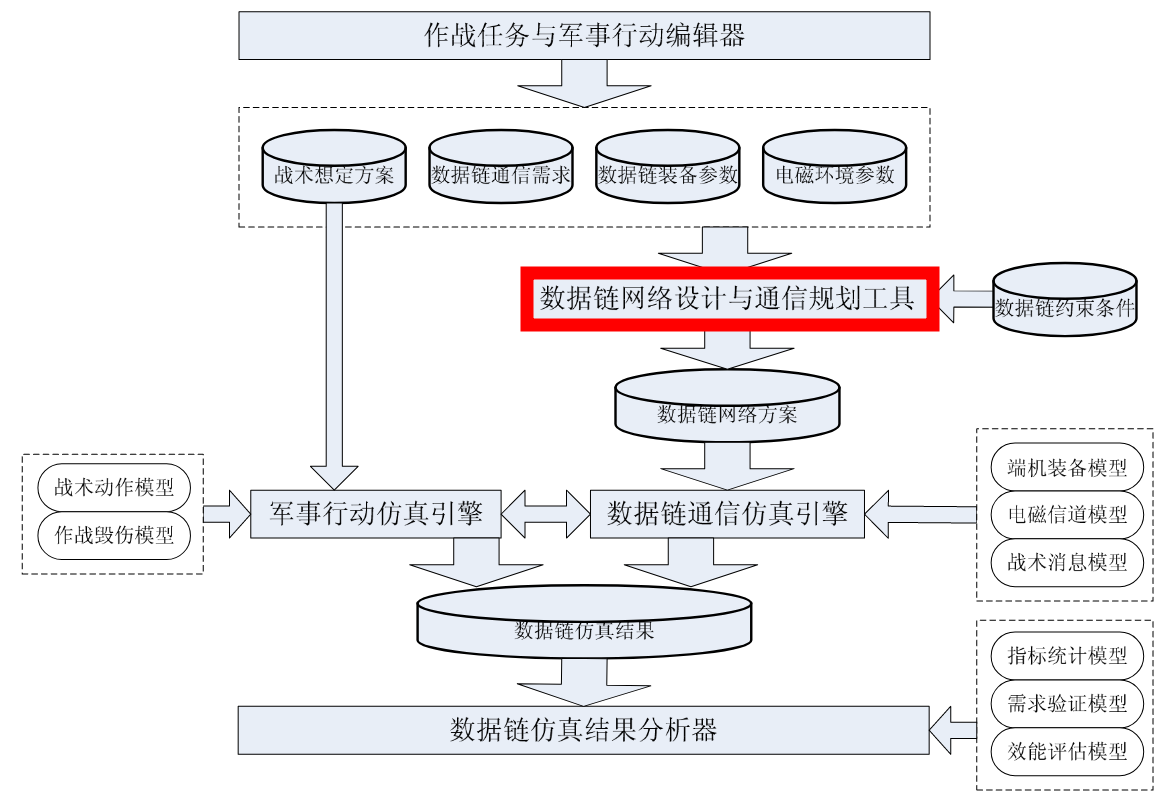
\includegraphics[width=1\linewidth]{./images/arch2.png}
		\end{figure}
	\end{spacing}
\end{frame}

\begin{frame}[fragile]
	\frametitle{战术数据链仿真平台框架}
	% \setlength{\parindent}{2em}
	\begin{spacing}{1.5}
		\begin{itemize}
			\item 军事行动仿真引擎: 根据战术想定方案, 驱动整个仿真系统按照给定
				的战术任务进行各项军事活动. 其中主要功能为根据作战任务与军事行动
				编辑器 生成的剧情, 调度推演作战战法的实现过程, 即是控制各个作战
				单元在某个时间 运动到某个地点, 发生某种作战动作, 触发某个战术信
				息报文的发送和接收, 从 而推动整个``剧情''往前推进. 
		\end{itemize}
	\end{spacing}
\end{frame}

\begin{frame}[fragile]
	\frametitle{战术数据链仿真平台框架}
	\setlength{\parindent}{2em}
	\begin{spacing}{1.5}
		\begin{figure}[htb]
			\centering
			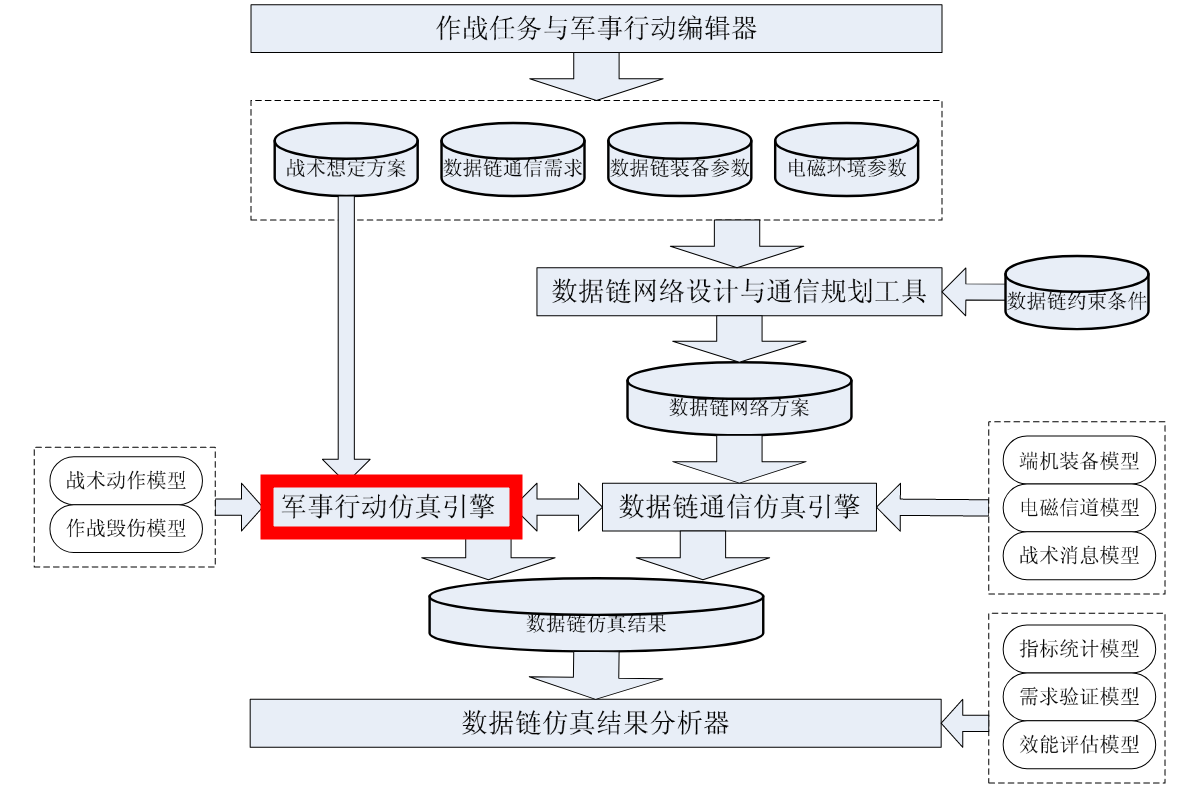
\includegraphics[width=1\linewidth]{./images/arch3.png}
		\end{figure}
	\end{spacing}
\end{frame} 

\begin{frame}[fragile]
	\frametitle{战术数据链仿真平台框架}
	% \setlength{\parindent}{2em}
	\begin{spacing}{1.5}
		\begin{itemize}
			\item 战术数据链通信仿真引擎: 取战术数据链组网设计规划工具产生的 组
				网方案, 利用各种仿真模型模拟仿真每一个战术消息报文的发送和接收过
				程,  触发各项军事活动以实现战术数据链军事行动仿真引擎交互, 记录
				每次报文发送 和接收的结果数据, 为战术数据链仿真结果分析器提供原
				始数据. 
		\end{itemize}
	\end{spacing}
\end{frame}

\begin{frame}[fragile]
	\frametitle{战术数据链仿真平台框架}
	\setlength{\parindent}{2em}
	\begin{spacing}{1.5}
		\begin{figure}[htb]
			\centering
			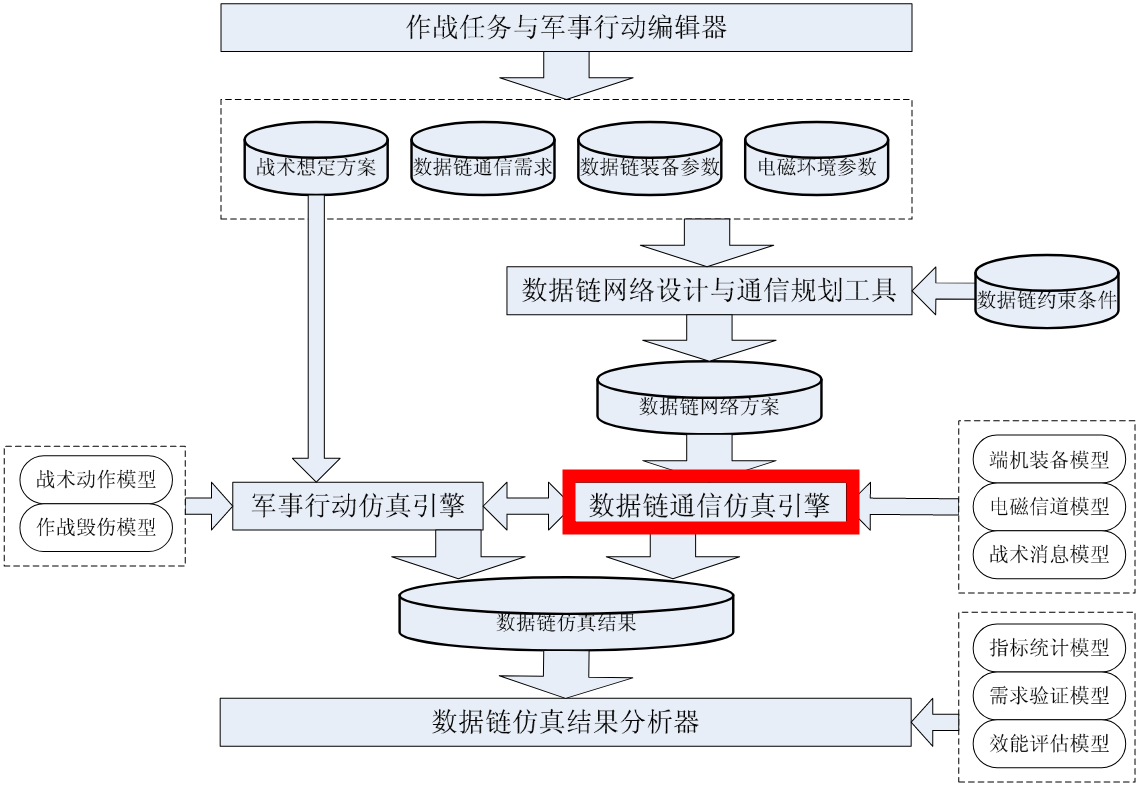
\includegraphics[width=1\linewidth]{./images/arch4.png}
		\end{figure}
	\end{spacing}
\end{frame}

\begin{frame}[fragile]
	\frametitle{战术数据链仿真平台框架}
	% \setlength{\parindent}{2em}
	\begin{spacing}{1.5}
		\begin{itemize}
			\item 战术数据链仿真结果分析器: 战术数据链仿真结果分析器, 主要根据军
				事行动仿真引擎和战术数据链通信 仿真引擎产生的仿真结果数据, 统计
				其中各项指标, 对照战术数据链信息交换需 求, 判断该组网方案是否能
				够满足给定战术任务的要求. 
		\end{itemize}
	\end{spacing}
\end{frame}

\begin{frame}[fragile]
	\frametitle{战术数据链仿真平台框架}
	\setlength{\parindent}{2em}
	\begin{spacing}{1.5}
		\begin{figure}[htb]
			\centering
			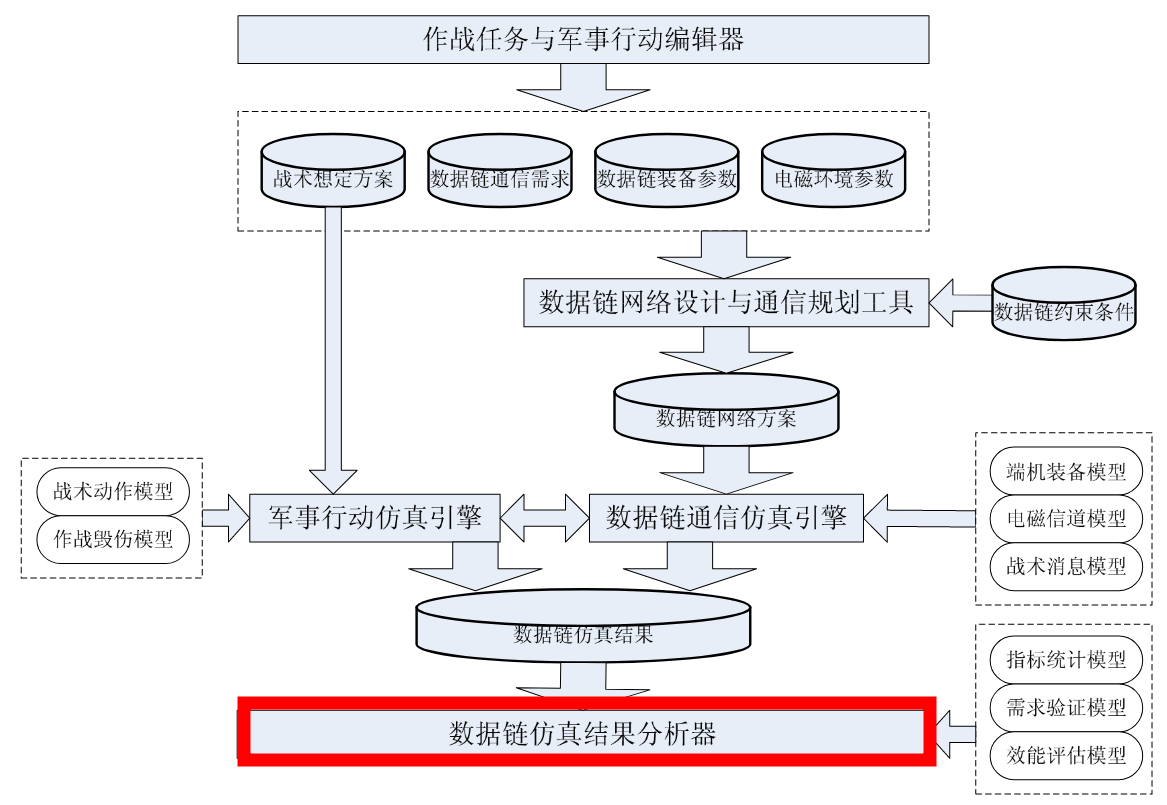
\includegraphics[width=1\linewidth]{./images/arch5.png}
		\end{figure}
	\end{spacing}
\end{frame}

\subsection{数据链通信仿真引擎}
\begin{frame}[fragile]
	\frametitle{数据链通信仿真引擎}
	\setlength{\parindent}{2em}
	\begin{spacing}{1.5}
		在上一章节提到的5个功能部件中, 数据链通信仿真引擎是整个仿真平台的核心部
		分, 其按照各个战术数据链装备终端信息发送和接收原理, 根据组网方案描述的装
		备平台初始化配置数据, 模拟仿真每一次战术信息报文在虚拟的战场环境中无线远
		距离传输. 

		该文章给出的仿真方案同样采用了分层模型的思路对整个通信系统做了拆解:
	\end{spacing}
\end{frame}

\begin{frame}[fragile]
	\frametitle{数据链通信仿真引擎}
	\setlength{\parindent}{2em}
	\begin{spacing}{1.5}
		该文章给出的仿真方案同样采用了分层模型的思路对整个通信系统做了拆解:
		\begin{figure}[htb]
			\centering
			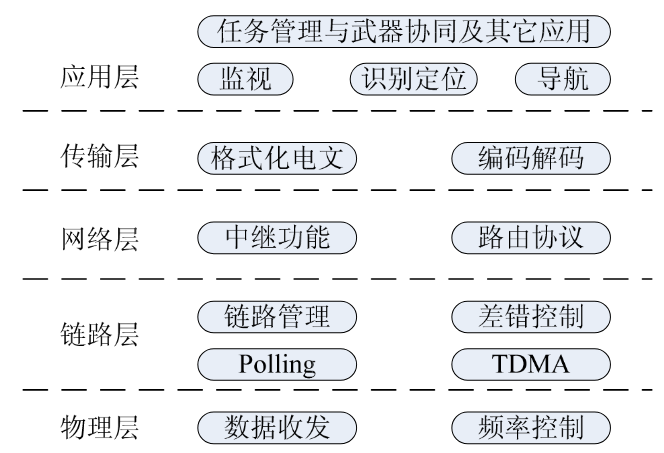
\includegraphics[width=0.8\linewidth]{./images/layer.png}
			\caption{战术数据链参考模型(TDLRM)}
			\label{Fig:layer}
		\end{figure}
	\end{spacing}
\end{frame}

\subsubsection{应用层}

\begin{frame}[fragile]
	\frametitle{应用层}
	\setlength{\parindent}{2em}
	\begin{spacing}{1.2}
		应用层主要规定了数据信息的结构、传输方法, 并规定了提供通信功能数据传输
		与操作的服务及协议, 根据具体规定来对不同信息组成的各种结构文件进行统
		一的处理. 应用层是解决操作系统平台和传输数据的融合, 实现数据的形象解析,
		便于任务控制和操作. 

		Link-16 战术数据链的应用层根据不同的战术应用划分多个网络参与组, 每个作
		战单元可以加入一个或多个网络参与组中, 支持各种战术任务要求. 其中三项重要
		的应用是:
		\begin{itemize}
			\item 雷达跟踪数据的共享, 以支持精确的态势感知;
			\item 精确参与定位与识别, 以向友军单元报告消息;
			\item 任务管理, 提供任务分配、目标报告给战斗机.
		\end{itemize}
		
		其他应用包括往返定时、语音通信和自由文本数据通信等等.
	\end{spacing}
\end{frame}

\begin{frame}[fragile]
	\frametitle{应用层}
	\setlength{\parindent}{2em}
	\begin{spacing}{1.5}
		\begin{figure}[htb]
			\centering
			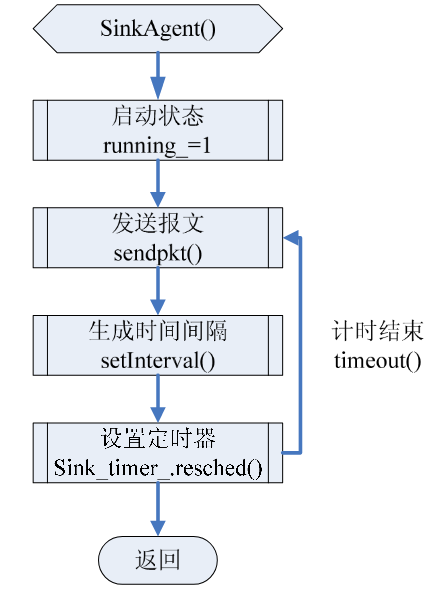
\includegraphics[width=0.5\linewidth]{./images/app.png}
			\caption{应用层定时器周期生产消息报文}
			\label{Fig:app}
		\end{figure}
	\end{spacing}
\end{frame}

\subsubsection{传输层}

\begin{frame}[fragile]
	\frametitle{传输层}
	\setlength{\parindent}{2em}
	\begin{spacing}{1.5}
		传输层是利用通信子网为两台端机的应用进程之间, 提供端到端的性能可靠、 透
		明传输的通信服务. 传输层最重要的两个传输层协议, 即无连接的 UDP 协议和 面
		向连接的 TCP 协议. 

		Link-16 战术数据链传输层提供传输媒介, 每个 NPG 的消息报文在特定的时隙组
		中以广播方式发送. 这些消息报文不包含目的地址(消息报文包含源地址).  同一
		网络中的任何接收机可以从一个特定 NPG 中接收与之有关的消息报文. 所以,
		Link-16 战术数据链的传输层既不是 UDP 也不是 TCP, 是广播方式发送消息, 功
		能比较简单. 
	\end{spacing}
\end{frame}

\subsubsection{网络层}

\begin{frame}[fragile]
	\frametitle{网络层}
	\setlength{\parindent}{2em}
	\begin{spacing}{1.5}
		网络层可以认为是端到端传输的最底层, 主要解决分组从源端沿着网络路径 送达
		目标端的路由协议的实现(包括地址编址方案)和算法的分析选择问题. 

		关于 Link-16 战术数据链的路由管理, 主要是通过泛洪算法来发现邻居, 将消息
		报文从源节点发送出去, 实现节点之间的通信. 
	\end{spacing}
\end{frame}

\begin{frame}[fragile]
	\frametitle{网络层}
	\setlength{\parindent}{2em}
	\begin{spacing}{1.5}
		\begin{figure}[htb]
			\centering
			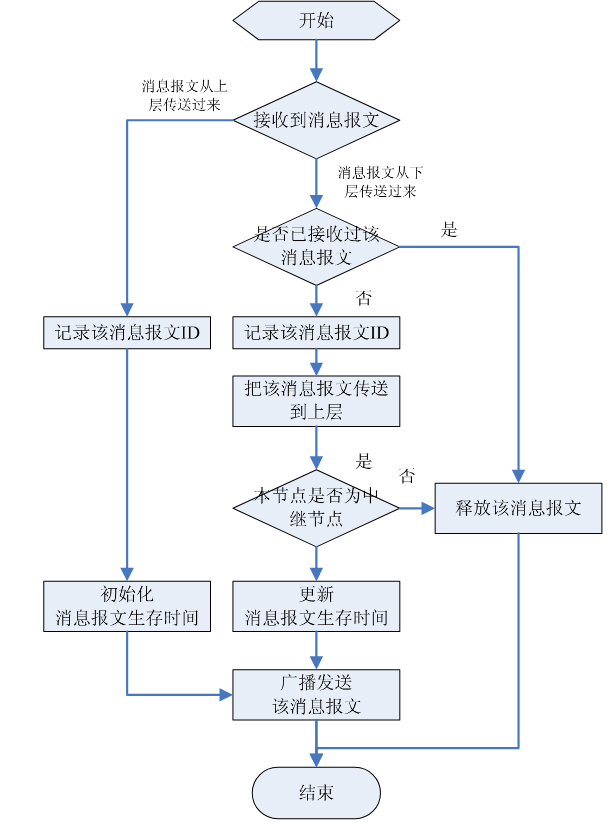
\includegraphics[width=0.6\linewidth]{./images/flood.png}
			\caption{基于洪泛方式的中继转发消息报文流程}
			\label{Fig:flood}
		\end{figure}
	\end{spacing}
\end{frame}

\subsubsection{链路层}

\begin{frame}[fragile]
	\frametitle{链路层}
	\setlength{\parindent}{2em}
	\begin{spacing}{1.5}
		数据链路层主要解决链路的建立、拆除、管理等功能, 以及数据的接入差错 控制
		等方面的问题; 数据链路层不仅能提供移动终端之间的逻辑连接, 还能提供 媒体
		访问的功能和用于连接处理的通信管理功能. 

		Link-16 战术数据链采用网络参与组的概念, 消息报文在链路层分类集合排队,
		做好发送前的准备, 以便选择适当的时隙发送出去. 由此可见, Link-16 的链路层
		从功能上来进一步细分, 可分为接口队列缓冲池(InterFace QueueS, IFqs)和媒介
		控制接入子层(Media Control Access, MAC). 
	\end{spacing}
\end{frame}

\begin{frame}[fragile]
	\frametitle{链路层}
	\setlength{\parindent}{2em}
	\begin{spacing}{1.5}
		\begin{figure}[htb]
			\centering
			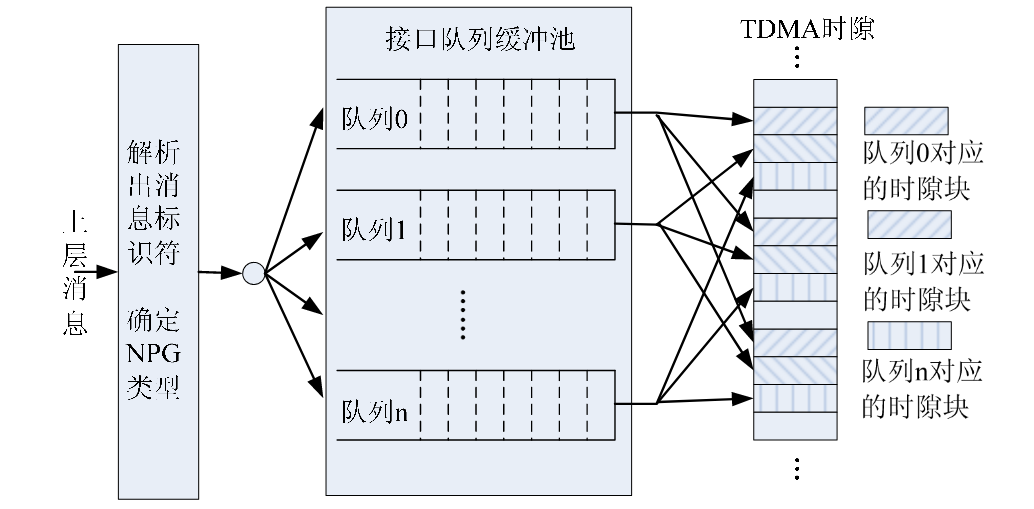
\includegraphics[width=0.9\linewidth]{./images/fifo.png}
			\caption{多队列缓冲池结构}
			\label{Fig:fifo}
		\end{figure}
	\end{spacing}
\end{frame}

\begin{frame}[fragile]
	\frametitle{链路层}
	\setlength{\parindent}{2em}
	\begin{spacing}{1.5}
		\begin{figure}[htb]
			\centering
			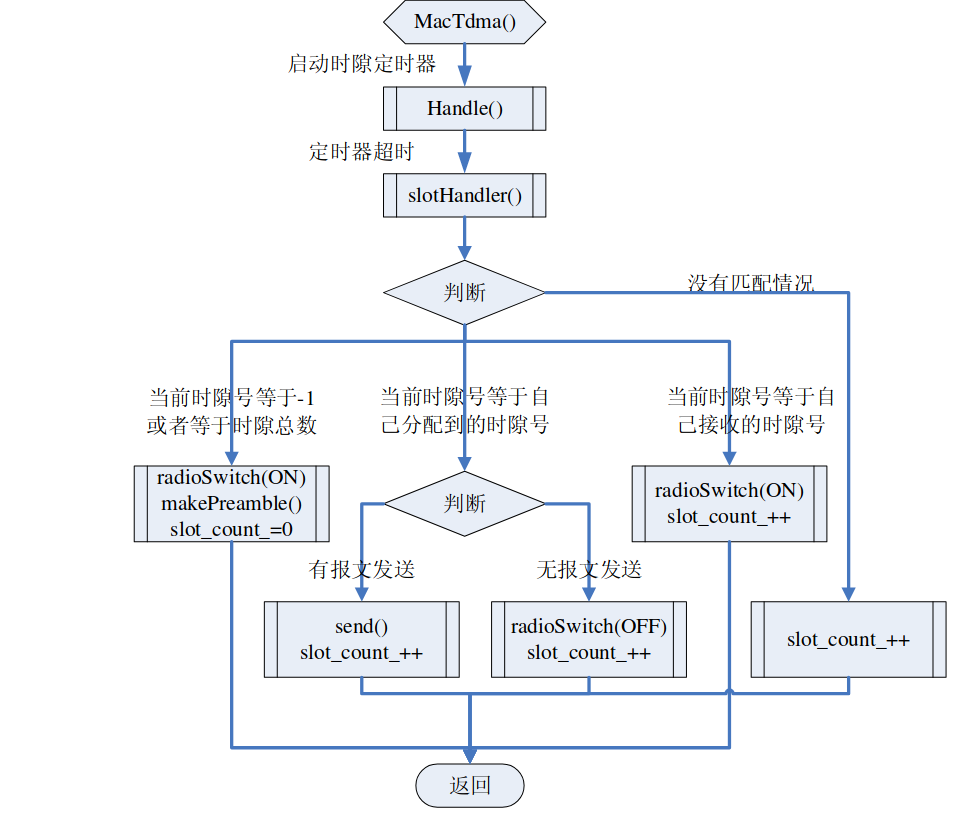
\includegraphics[width=0.8\linewidth]{./images/tdma.png}
			\caption{TDMA协议的关键时隙控制执行过程}
			\label{Fig:mac}
		\end{figure}
	\end{spacing}
\end{frame}

\subsubsection{物理层}
\begin{frame}[fragile]
	\frametitle{物理层}
	\setlength{\parindent}{2em}
	\begin{spacing}{1.5}
		物理层负责频率选择, 接收和发送链路层的信息, 确定定时位同步信息, 同 时解
		决通信平台和数据传输线路之间的连接协议和接口问题.

	\end{spacing}
\end{frame}

\begin{frame}[fragile]
	\frametitle{物理层}
	\setlength{\parindent}{2em}
	\begin{spacing}{1.5}
		Link-16 战术数据链系统通过多网结构的工作方式来达到系统扩充容量的目的.
		每个网络单元在参与的不同的网络参与组中处在不同的网络, 相当于处在多个互不
		干扰的无线信道之一, 这样使得不同网络参与组的多个成员可以使用同一组时隙工
		作. 

		\begin{figure}[htb]
			\centering
			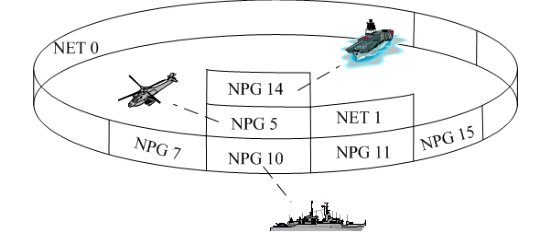
\includegraphics[width=0.8\linewidth]{./images/multi.png}
			\caption{Link-16多网结构}
			\label{Fig:multi}
		\end{figure}
	\end{spacing}
\end{frame}

\begin{frame}[fragile]
	\frametitle{物理层}
	\setlength{\parindent}{2em}
	\begin{spacing}{1.5}
		为了提高系统传输的抗干扰性, Link-16 战术数据链采用了跳频技术. 在每个单网
		结构(或是单个无线信道)中, 消息报文的波形在 Lx 波段960MHz\~1215MHz 上 51
		个离散的载波频率上均匀分布并以 76923Hop/s 的跳频速率快速跳变. 

		\begin{figure}[htb]
			\centering
			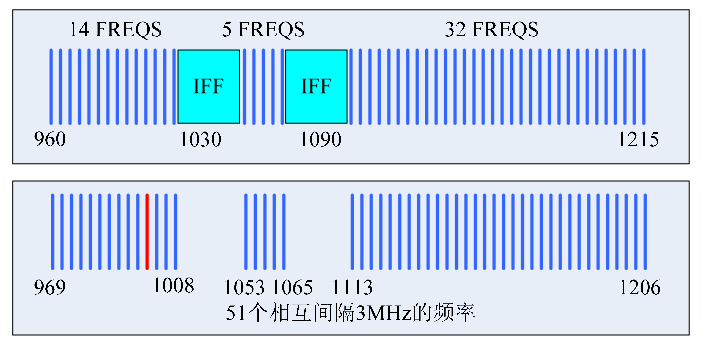
\includegraphics[width=0.8\linewidth]{./images/jump.png}
			\caption{Link-16跳频技术}
			\label{Fig:jump}
		\end{figure}
	\end{spacing}
\end{frame}

\begin{frame}[fragile]
	\frametitle{物理层}
	\setlength{\parindent}{2em}
	\begin{spacing}{1.5}
		\begin{figure}[htb]
			\centering
			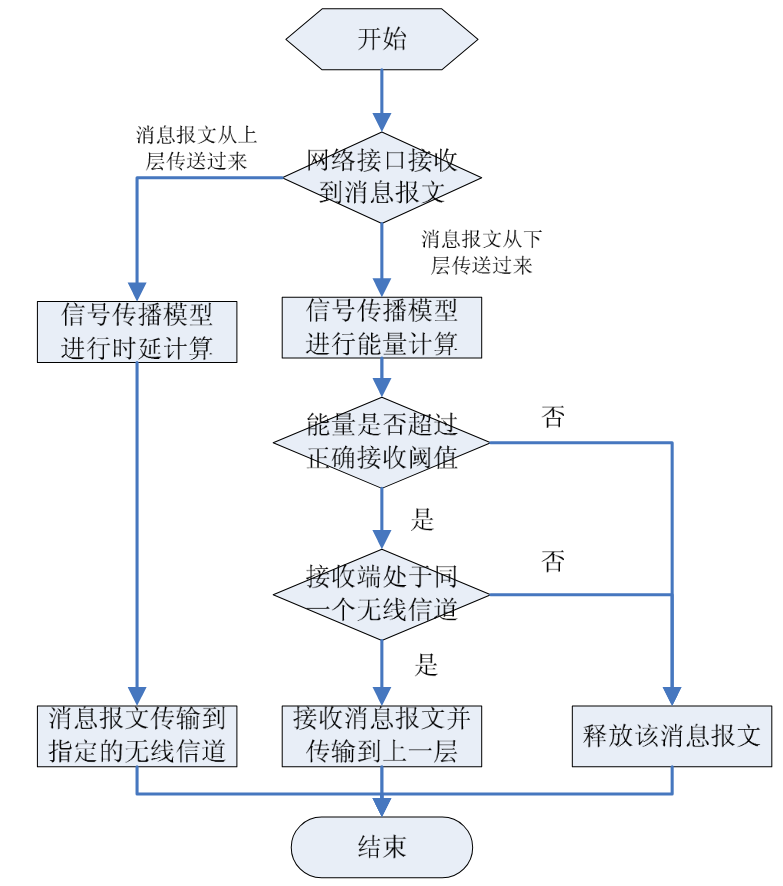
\includegraphics[width=0.6\linewidth]{./images/phy.png}
			\caption{多信道跳频收发消息流程}
			\label{Fig:phy}
		\end{figure}
	\end{spacing}
\end{frame}

\section{仿真方式与流程}

\begin{frame}[fragile]
	\frametitle{仿真方式与流程}
	% \setlength{\parindent}{2em}
	\begin{spacing}{1.5}
		总的来说, 仿真的流程如下:
		\begin{enumerate}
			\item 根据战术任务实施区域(即作战区域)的大小配置仿真场景的大小;
			\item 根据战术任务实施过程参战单元的数量、类型以及地理位置部署配置网
				络拓扑;
			\item 根据战术任务实施过程所拟定的作战方案(其中包括各参战单元移动
				方 向和速度等)配置节点的移动性;  
			\item 根据战术任务所要求的网络参与群数量、类型以及各网络参与群的
				参与 节点相应地配置网络功能;  
			\item 根据信息交换需求所拟定的各节点发送战术消息的类型、时间、速
				率以及数据量大小等配置各个节点的消息流量;  
		\end{enumerate}
	\end{spacing}
\end{frame}

\begin{frame}[fragile]
	\frametitle{仿真方式与流程}
	\setlength{\parindent}{2em}
	\begin{spacing}{1.3}
		\begin{enumerate}
			\item[6.] 通过选择合适的节点担任相应的网络职责(如网络时间基准和中继节
				点 等)配置网络角色;  
			\item[7.] 将时间、频率和信道等网络资源具体分配到每个节点实现网络资源
				的配置;  
			\item[8.] 通过设置障碍、噪声和干扰等来配置作战环境; 
			\item[8.] 设置各个节点所装备的终端平台类型, 确定其天线类型、调制方式、
				带宽和功率等, 配置好通信终端;  
			\item[10.] 根据终端平台类型确定信道接入方式(如 Link-11 战术数据链的轮
				询方式与 Link-16 战术数据链的 TDMA 专用/竞争方式), 配置通信协议;  
			\item[11.] 通过对仿真时间、随机种子数等的配置, 运行仿真, 并对相关数据
				进行统计;  
			\item[12.] 根据仿真需求, 对结果进行分析, 并输出相应指标的分析结果, 包
				括时延、时延抖动、丢失率等. 
		\end{enumerate}
	\end{spacing}
\end{frame}

\section{目前进度与方向}
\begin{frame}[fragile]
	\frametitle{目前进度与方向}
	\setlength{\parindent}{2em}
	\begin{spacing}{1.5}
		\begin{itemize}
			\item 正学习利用ns-3搭一个简易的数据链通信仿真引擎的demo出来, 暂时不
				考虑军事行动编辑器、行动仿真引擎、结果分析器等框架中的其余组件.
				\begin{itemize}
					\item 在通信引擎内部, 考虑暂时跳过一些具体的技术细节, 先把参
						考分层模型的几层结构都搭建出来, 保留好用于拓展的接口, 以
						便后续添加细节.
				\end{itemize}
			\item 仿真的可视化模块也暂时不考虑.
		\end{itemize}
	\end{spacing}
\end{frame}


\section{参考文献}
\begin{frame}{参考文献}
    \begin{tiny}
        \bibliographystyle{unsrt}
        \bibliography{ref}
    \end{tiny}
\end{frame}


{\xdbg%末页致谢
\begin{frame}[plain,noframenumbering]
 \finalpage{{\huge 感谢观看!}}
\end{frame}}

\end{document} 
